\documentclass[runningheads]{llncs}

\usepackage{graphicx}
\usepackage{listings}
\usepackage{hyperref}
% Used for displaying a sample figure. If possible, figure files should
% be included in EPS format.
%
% If you use the hyperref package, please uncomment the following line
% to display URLs in blue roman font according to Springer's eBook style:
\renewcommand\UrlFont{\color{blue}\rmfamily}

% tablespacing
\renewcommand{\arraystretch}{1.5}
\setlength\tabcolsep{0.2cm}

% Copyright 2017 Sergei Tikhomirov, MIT License
% https://github.com/s-tikhomirov/solidity-latex-highlighting/

\usepackage{listings, xcolor}

\definecolor{verylightgray}{rgb}{.97,.97,.97}

\lstdefinelanguage{Solidity}{
	keywords=[1]{anonymous, assembly, assert, balance, break, call, callcode, case, catch, class, constant, continue, contract, debugger, default, delegatecall, delete, do, else, emit, event, export, external, false, finally, for, function, gas, if, implements, import, in, indexed, instanceof, interface, internal, is, length, library, log0, log1, log2, log3, log4, memory, modifier, new, payable, pragma, private, protected, public, pure, push, require, return, returns, revert, selfdestruct, send, storage, struct, suicide, super, switch, then, this, throw, transfer, true, try, typeof, using, value, view, while, with, addmod, ecrecover, keccak256, mulmod, ripemd160, sha256, sha3}, % generic keywords including crypto operations
	keywordstyle=[1]\color{blue}\bfseries,
	keywords=[2]{address, bool, byte, bytes, bytes1, bytes2, bytes3, bytes4, bytes5, bytes6, bytes7, bytes8, bytes9, bytes10, bytes11, bytes12, bytes13, bytes14, bytes15, bytes16, bytes17, bytes18, bytes19, bytes20, bytes21, bytes22, bytes23, bytes24, bytes25, bytes26, bytes27, bytes28, bytes29, bytes30, bytes31, bytes32, enum, int, int8, int16, int24, int32, int40, int48, int56, int64, int72, int80, int88, int96, int104, int112, int120, int128, int136, int144, int152, int160, int168, int176, int184, int192, int200, int208, int216, int224, int232, int240, int248, int256, mapping, string, uint, uint8, uint16, uint24, uint32, uint40, uint48, uint56, uint64, uint72, uint80, uint88, uint96, uint104, uint112, uint120, uint128, uint136, uint144, uint152, uint160, uint168, uint176, uint184, uint192, uint200, uint208, uint216, uint224, uint232, uint240, uint248, uint256, var, void, ether, finney, szabo, wei, days, hours, minutes, seconds, weeks, years},	% types; money and time units
	keywordstyle=[2]\color{teal}\bfseries,
	keywords=[3]{block, blockhash, coinbase, difficulty, gaslimit, number, timestamp, msg, data, gas, sender, sig, value, now, tx, gasprice, origin},	% environment variables
	keywordstyle=[3]\color{violet}\bfseries,
	identifierstyle=\color{black},
	sensitive=false,
	comment=[l]{//},
	morecomment=[s]{/*}{*/},
	commentstyle=\color{gray}\ttfamily,
	stringstyle=\color{red}\ttfamily,
	morestring=[b]',
	morestring=[b]"
}

\lstset{
	language=Solidity,
	backgroundcolor=\color{verylightgray},
	extendedchars=true,
	basicstyle=\footnotesize\ttfamily,
	showstringspaces=false,
	showspaces=false,
	numbers=left,
	numberstyle=\footnotesize,
	numbersep=9pt,
	tabsize=2,
	breaklines=true,
	showtabs=false,
	captionpos=b
}


\lstset{basicstyle=\small\ttfamily}

\begin{document}
%
\title{Untrusted B2B Collaboration using the Blockchain}
%
%
\author{Jonas Beyer \and Philipp Otto \and S\"oren Tietb\"ohl}
%
\authorrunning{J. Beyer et al.}
%
\institute{
	Hasso-Plattner-Institut, Potsdam, Germany\\
	\email{\{jonas.beyer,philipp.otto2,soeren.tietboehl\}@student.hpi.de}}
%
\maketitle % typeset the header of the contribution
%
\begin{abstract}
	Lack of trust between communication partners is one of the major issues companies face when implementing business processes in a cross-organizational setting.
	Blockchain is an emerging technology that enables decentralization and distribution of state without the need for a trusted central instance.
	As a result, it is possible to form consensus in the communication between otherwise untrusting parties.
	In this paper we introduce Armadillo, an open-source prototype implementation for realizing business process choreographies using the Ethereum blockchain.
	We present smart contract system for inter-process communication, as well as a user interface for connecting business processes and smart contracts.
	While our solution is not production-ready in terms of transaction costs, it describes a basis for untrusted messaging via the blockchain without a central controlling party.

	\keywords{Business Processes \and BPMN \and Choreographies \and Blockchain \and Ethereum \and Smart Contracts}
\end{abstract}
%
\section{Introduction}
% BPM
Business Process Management (BPM) allows organizations to identify, structure and understand the tasks and processes they employ to achieve their business goals.
%Process Models
In BPM, Process models are used to document how these goals can be reached, visually describing the participants, activity flow and data objects involved.
By sharing process models with their employees, organizations can ensure a common understanding of the work that needs to be done.

% What is BPMN?
Business Process Model and Notation (BPMN) is a standard notation for process models~\cite{omg2014bpmn}.
It provides building blocks for the modeling of complex intra- and inter-business processes.
As BPM is not limited internal procedures, but also considers communication with external partners, BPMN can be used to model the message exchange needed for sucessful cooperation.

% Trust
The basis for inter-process communication is that all involved parties trust each other.
Companies can enter contracts to safeguard themselves against possibly malicious partners, but it can still lead a lot of overhead to claim their rights in case of a contract infringement.
Further problems arise when multiple parties are involved in a process:
The more partners there are, the more difficult it becomes to track faults and misunderstandings in the communication.

% What is Blockchain?
With the help of the emerging Blockchain technology, these problems can be resolved.
A Blockchain is a decentralized information storage network.
Information is stored in blocks, which are chained together via cryptograhic means.
In this network, many participants can agree on a public common state of information without trusting each other.
Blockchain technology is commonly used to realize virtual currencies, also called cryptocurrencies.
Ethereum~\cite{wood2014ethereum} is one implementation of the Blockchain concept which also realizes a feature called smart contracts.
Smart contracts are small programs that are executed by the nodes in the Blockchain network.
They have very limited processing power, but they enable the execution of code which has a commonly known state.

%What problems are there with BPMN that can be solved with Blockchain?
Blockchain features can be used to facilitate trusted communication between untrusted parties in Business Process Management.
% What approaches exist currently (Caterpillar~\cite{lopez2017caterpillar}, Untrusted paper~\cite{weber2016untrusted})
Existing approaches aim to bring BPM functionality to the Ethereum Blockchain utilizing smart contracts.
Weber et al.~\cite{weber2016untrusted}, e.g., realize process orchestrations on the Blockchain using a smart contract as the mediator for messages and execution state.
% What is our general Idea?
We expand on the work of Weber et al. and implement process choreographies, where instead of one central mediator, each party provides their own smart contracts.
Communication then happens directly between the partner's contracts instead of going through a central instance.

% Structure
The rest of this paper is structured as follows: In Section \ref{preliminary} we will discuss concepts and technologies required for our work, and introduce our use case.
In Section \ref{solutionapproach} we will present the solution requirements and concepts.
Section \ref{implementation} describes our contract and tool implementations.
In Section \ref{evaluation} we evaluate our solution.
Finally, Section \ref{futurework} will present future work and Section \ref{conclusion} will conclude the paper.

\section{Preliminary} \label{preliminary}

In the following section we present concepts and technologies that are related to our work.

\subsection{Business Process Collaboration}

When businesses work together to reach a common goal, their processes also need to comply with each other.
Such business-to-business collaborations can also be modeled in BPMN.
Collaboration models include the businesses' \emph{public processes} (or \emph{behavioral interfaces}~\cite{Weske2012}), i.e., the BPMN tasks and events describing the sending and receiving of messages, as well as the message flow between the participants.
While not directly part of the interaction, they can also depict \emph{private processes}, i.e., tasks and control flows that are internally executed before or after sending or receiving a message.
An example can be seen in Figure \ref{fig:collaboration}.

Process interoperability needs to be ensured when it comes to executing a collaboration model.
To this end, there are two different implementation approaches:
One option is to treat the collaboration like a local, internal process, employing a \emph{process orchestration}.
In a process orchestration, the execution is controlled by a central instance.
Adopting the role of a mediator or manager, this central instance dictates and guides the execution.
Thus, the execution has a well-defined order of tasks and a clear execution state.

Another option is to have the participants act more independently.
In \cite{Weske2012}, Weske describes \emph{process choreographies}, which define and ensure a set of collaboration rules to ensure interoperabiltiy.
A choreography clarifies the dependencies between the participant's processes and the messages they need to exchange for a successful collaboration.
Communication and execution is not handled by a central instance, but rather by each participant on their own.
Messages are passed asynchronously without a controlling channel.
As a result, there is no clear execution state, because each participant drives their own execution.

\subsection{Blockchain}

A blockchain is a distributed ledger that allows users to find a consensus in decentralized applications.
Information is stored in a linked list of blocks and shared between all participants, i.e., all nodes in a decentralized computer network.
By only allowing new blocks to be appended to the list, a non-rewritable history is created, that at the same time represents the "truth", the common state all nodes in the network agree on.
There are multiple approaches of determining who is allowed to append a new block, altering the state.
The most common one, currently employed for example by Bitcoin~\cite{nakamoto2008bitcoin} and Ethereum~\cite{wood2014ethereum}, is called \emph{proof of work}:
Each new block has to contain a signature that verifies the block order.
The signature is created using data from the preceding block and is by design mathematically hard to calculate, but easy to verify.
On the one hand, this results in a race between so called \emph{mining} nodes who try and calculate such a signature, as the first valid signature verifies the new block's position and stores it's data on the ledger.
Mining nodes get rewarded for finding such signatures, creating an incentive for continuous appending of new blocks and keeping the blockchain alive.
On the other hand, other nodes can easily verify the signature and come to a consensus regarding the latest state.
If the same block is signed at the same time, a fork of the blockchain is created, where two versions of the blockchain exist at the same time.
Consensus is then reached when new blocks are appended, propagating the longest blockchain within the network until it is accepted by all parties.

Blockchain technology is mainly used for cryptocurrencies, most notably Bitcoin~\cite{nakamoto2008bitcoin}.
In more recent developments however, they are used as a foundation for a number of other decentralized applications.
Ethereum~\cite{wood2014ethereum} is a platform that uses a blockchain as the underlying system, but further allows users write and execute code in the form of \emph{smart contracts}.
Smart contracts are Turing complete code artifacts that can be deployed on the blockchain and are accessible by accounts in the Ethereum platform.
When called by a user account or another contract, they can perform calculations, send or receive money, or store information on the blockchain ledger either directly or in the form of \emph{events}.
Events are publicly visible and can be watched by off-chain applications, allowing external programs to react to blockchain state changes.
This would otherwise not be possible, ss smart contracts can not communicate with anything outside the blockchain.

When calling functions on a smart contract, users have to supply \emph{gas}, a unit that powers smart contract computations.
Contracts deplete gas for each operation and return excess gas back to the user.
This ensures that contracts are not running for an unlimited amount of time, avoiding a dead lock of the platform.
Computations on the blockchain are expensive in order to avoid unnecessary operations, as all operations have to be performed by each node in the network.
Because of the gas limit and high execution cost, the computational power of smart contracts is limited.

Smart contracts are executed in the \emph{Ethereum virtual machine (EVM)}.
As such, they contain byte code that is interpreted by the VM.
When developing smart contracts, there are multiple languages that compile to EVM bytecode, the most prominent one currently being \emph{Solidity}\footnote{\url{https://github.com/ethereum/solidity}}, which we also chose to implement our protoype.
Xu et al. present patterns and examples for Solidity programming in~\cite{xu2018pattern}, which we used as orientation during development.

\subsection{Prior Work on Business Processes on the Blockchain}
In~\cite{weber2016untrusted}, a first approach of monitoring and coordinating business process interactions across organizations on the blockchain was presented.
Using a smart contract as a central \emph{monitor} or \emph{mediator} of the communication, a form of inter-process orchestration is implemented.
The mediator is also responsible for role management, i.e., participants can register users to certain roles with the mediator, who verifies these roles at runtime.
The architecture features factory contracts, which are responsible for deploying instance contracts for each process instance.
For integrating blockchain and BPM applications, the concept of \emph{triggers} is introduced: Applications that watch events on the blockchain and trigger external API calls.

We built our implementation based on these concepts.
However, our solution differs from the solution in~\cite{weber2016untrusted} in the way we realize the execution of collaboration models.
As stated before, Weber et al. employ the central mediator contract, managing execution steps and internal state of the collaboration, achieving the orchestration of a business process collaboration.
Our goal on the other hand was to implement the collaboration as a choreography, where each participant is represented by their own contracts, and is able to verify the integrity of their interaction partners.
Thus, a central mediator is no longer needed, also resolving the question of who is responsible for the development, deployment and maintenance of the mediator contract.

In order to achieve BPMN-to-Solidity compilation,~\cite{weber2016untrusted} also describes translation rules to transform BPMN elements to Solidity code.
Further work~\cite{banuelos2017optimized} tries to optimize the translation process, in turn reducing Ethereum execution costs by reducing required space and operations.

We have not made an automated translation our primary goal.
Instead, we focussed on designing an architecture that allows for the above mentioned choreography implementation.
However, we believe that an at least semi-automatic translation process can be derived from our results.

Caterpillar~\cite{lopez2017caterpillar} is an open source implementation of a process engine using smart contracts, handling the most common BPMN elements.
Building on the BPMN-to-Solidity compilation from~\cite{weber2016untrusted}, it integrates translation, deployment and execution of BPMN models in the form of smart contracts directly on the Ethereum Blockchain.
It also allows a translation of BPMN Models to smart contracts, which can be deployed and executed directly on the Ethereum Blockchain.
Processes can be started and executed via a user interface, which encapsulates the calls the generated Solidity code in the background.

Our approach is different in that we do not try to use the Ethereum platform as a process engine, but rather use it only for message passing, and integrate it with an off-chain process engine.
Caterpillar also currently does not support the execution of process interactions.

\subsection{Use Case}

Since we build on a lot of the work in~\cite{weber2016untrusted}, we decided to also continue with the example collaboration\footnote{A supply chain scenario reported originally in~\cite{fdhila2015collaborative}, which was simplified in~\cite{weber2016untrusted}.} used there.
Because we implemented contracts for each participant, we needed to expand the collapsed pool for the \emph{Bulk Buyer}, and add tasks and events for the corresponding public process.
We added a new lane to the \emph{Manufacturer's} process for demonstration of the role management we implemented.
The result is depicted in Figure \ref{fig:collaboration}.

When we present the implementation, the tasks that are modeled as BPMN message sends in the collaboration model will instead be modeled as \emph{BPMN service tasks} in the separate processes.
This decision is based on the notion that in our implementation, all sends are a call to the Ethereum platform, which acts as the external service and takes over the actual messaging.
This implementation detail is not relevant in the collaboration view, though, where we are concerned with the interactions.

\begin{figure}
	\centering
	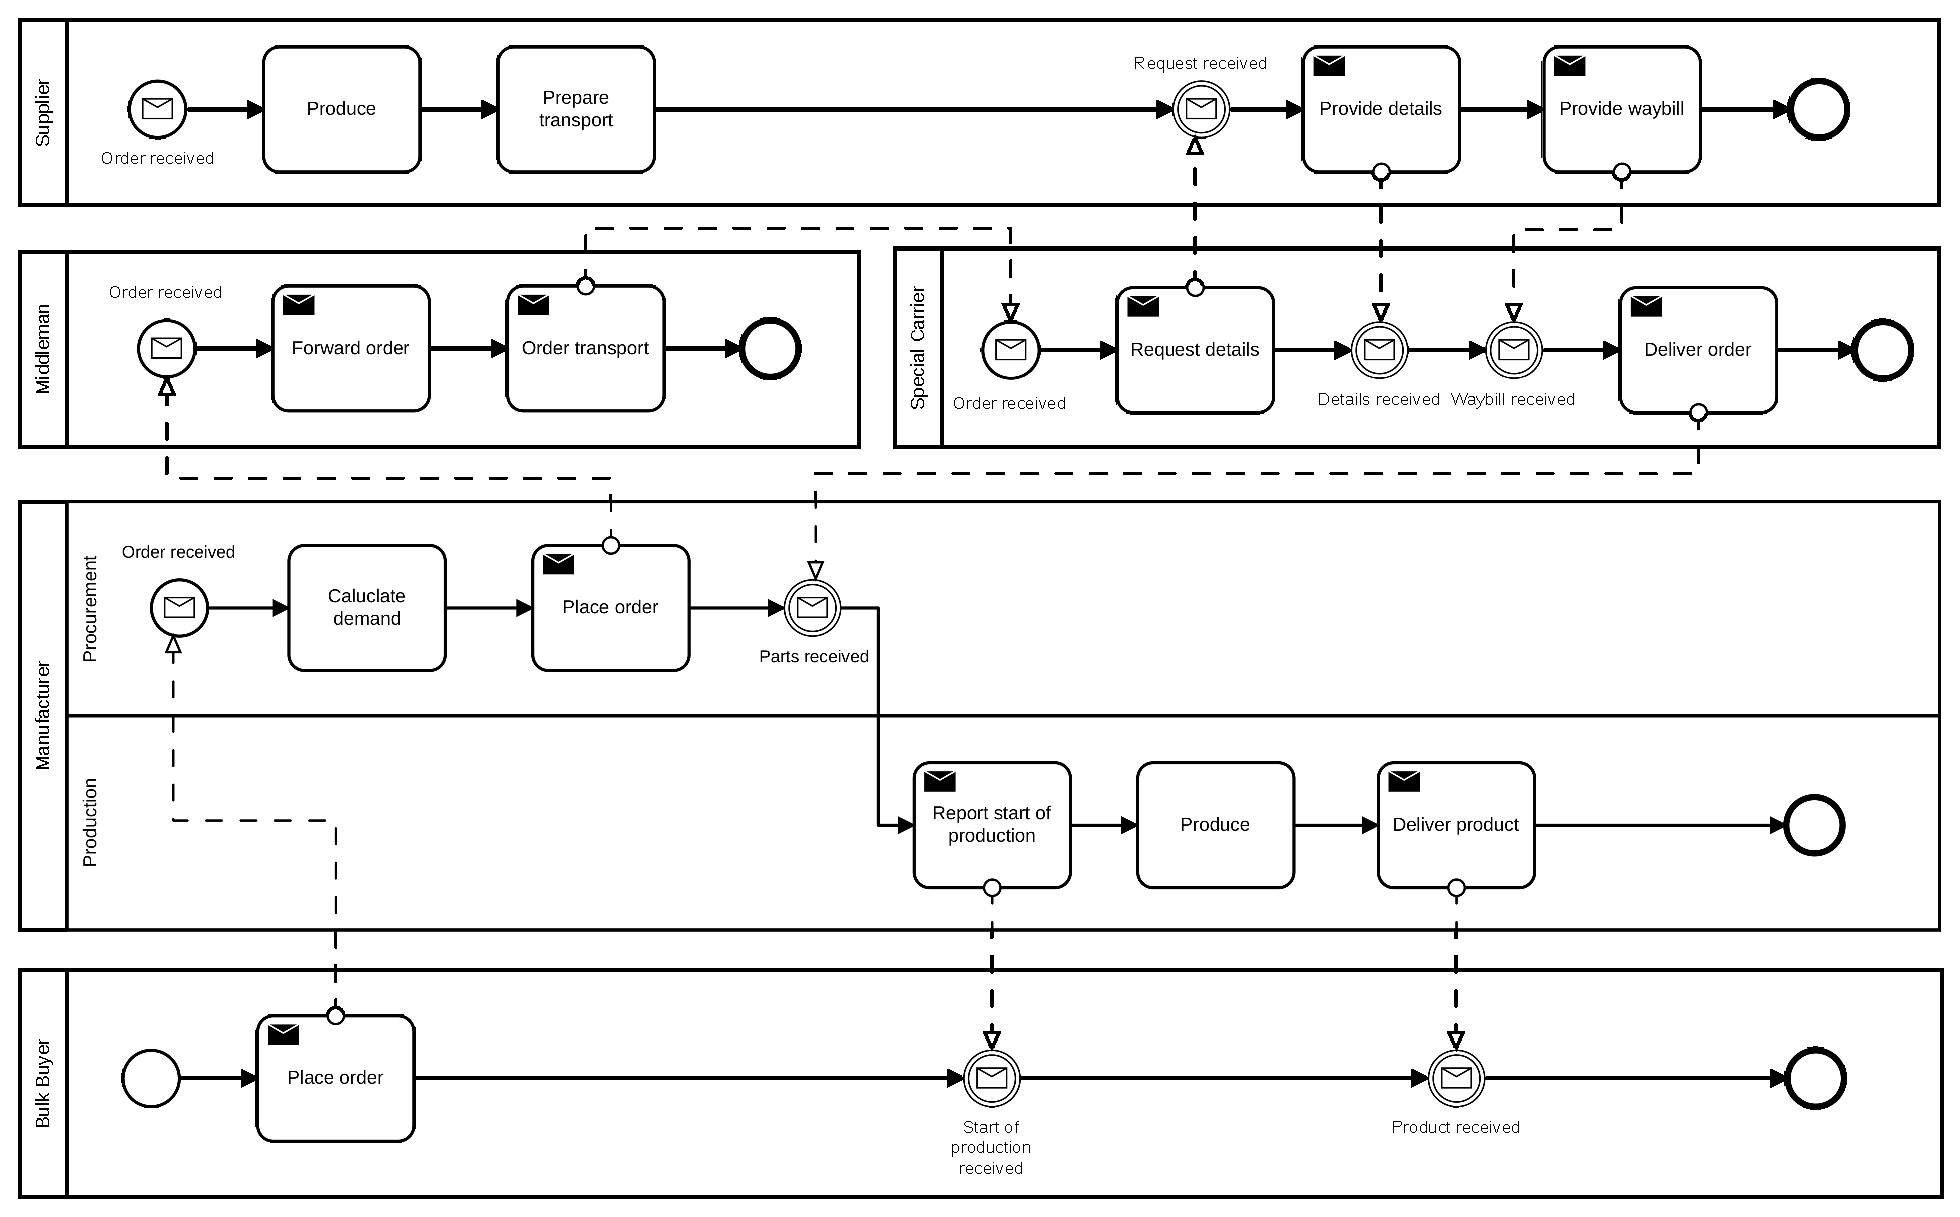
\includegraphics[width=\textwidth]{fig/collaboration.eps}
	\caption{Supply chain scenario from~\cite{weber2016untrusted} (modified).}
	\label{fig:collaboration}
\end{figure}

\section{Solution Approach} \label{solutionapproach}
We propose a system design, that allows choreographies to be executed publicly on the blockchain.
In the following section, we describe our approach and its architecture.

\subsection{Requirements}

Before presenting the system, want to give an overview of the functional and non-functional requirements it has to fulfill.

The system's purpose is to facilitate trusted communication and collaboration between untrusting partners.
Therefore, it must be possible to send messages between partners.
To ensure security and trust in the system, both partners need a way to verify the authenticity of a message.
Verification is only possible if the system keeps track of users and permissions, i.e., implements a form of role-based access control with a user-to-role and role-to-permission mapping.
User and permission data has to be accessible at runtime, so that the communicating partners can use it to check the authenticity of messages.
It should also be possible to modify this data at runtime, to accomodate for changes in the company structure.

In order to make this system feasible in a production environment, we also require it to be reusable, measurable and cheap.
This implies keeping the implementation small and modular, and keeping it general enough to be used with the processes of different participants.
Measurability is required for evaluation and monitoring.
Since all computation done by smart contracts comes with gas costs, we want to keep the cost of our implementation as low as possible.

\subsection{System Overview}
\begin{figure}
	\centering
	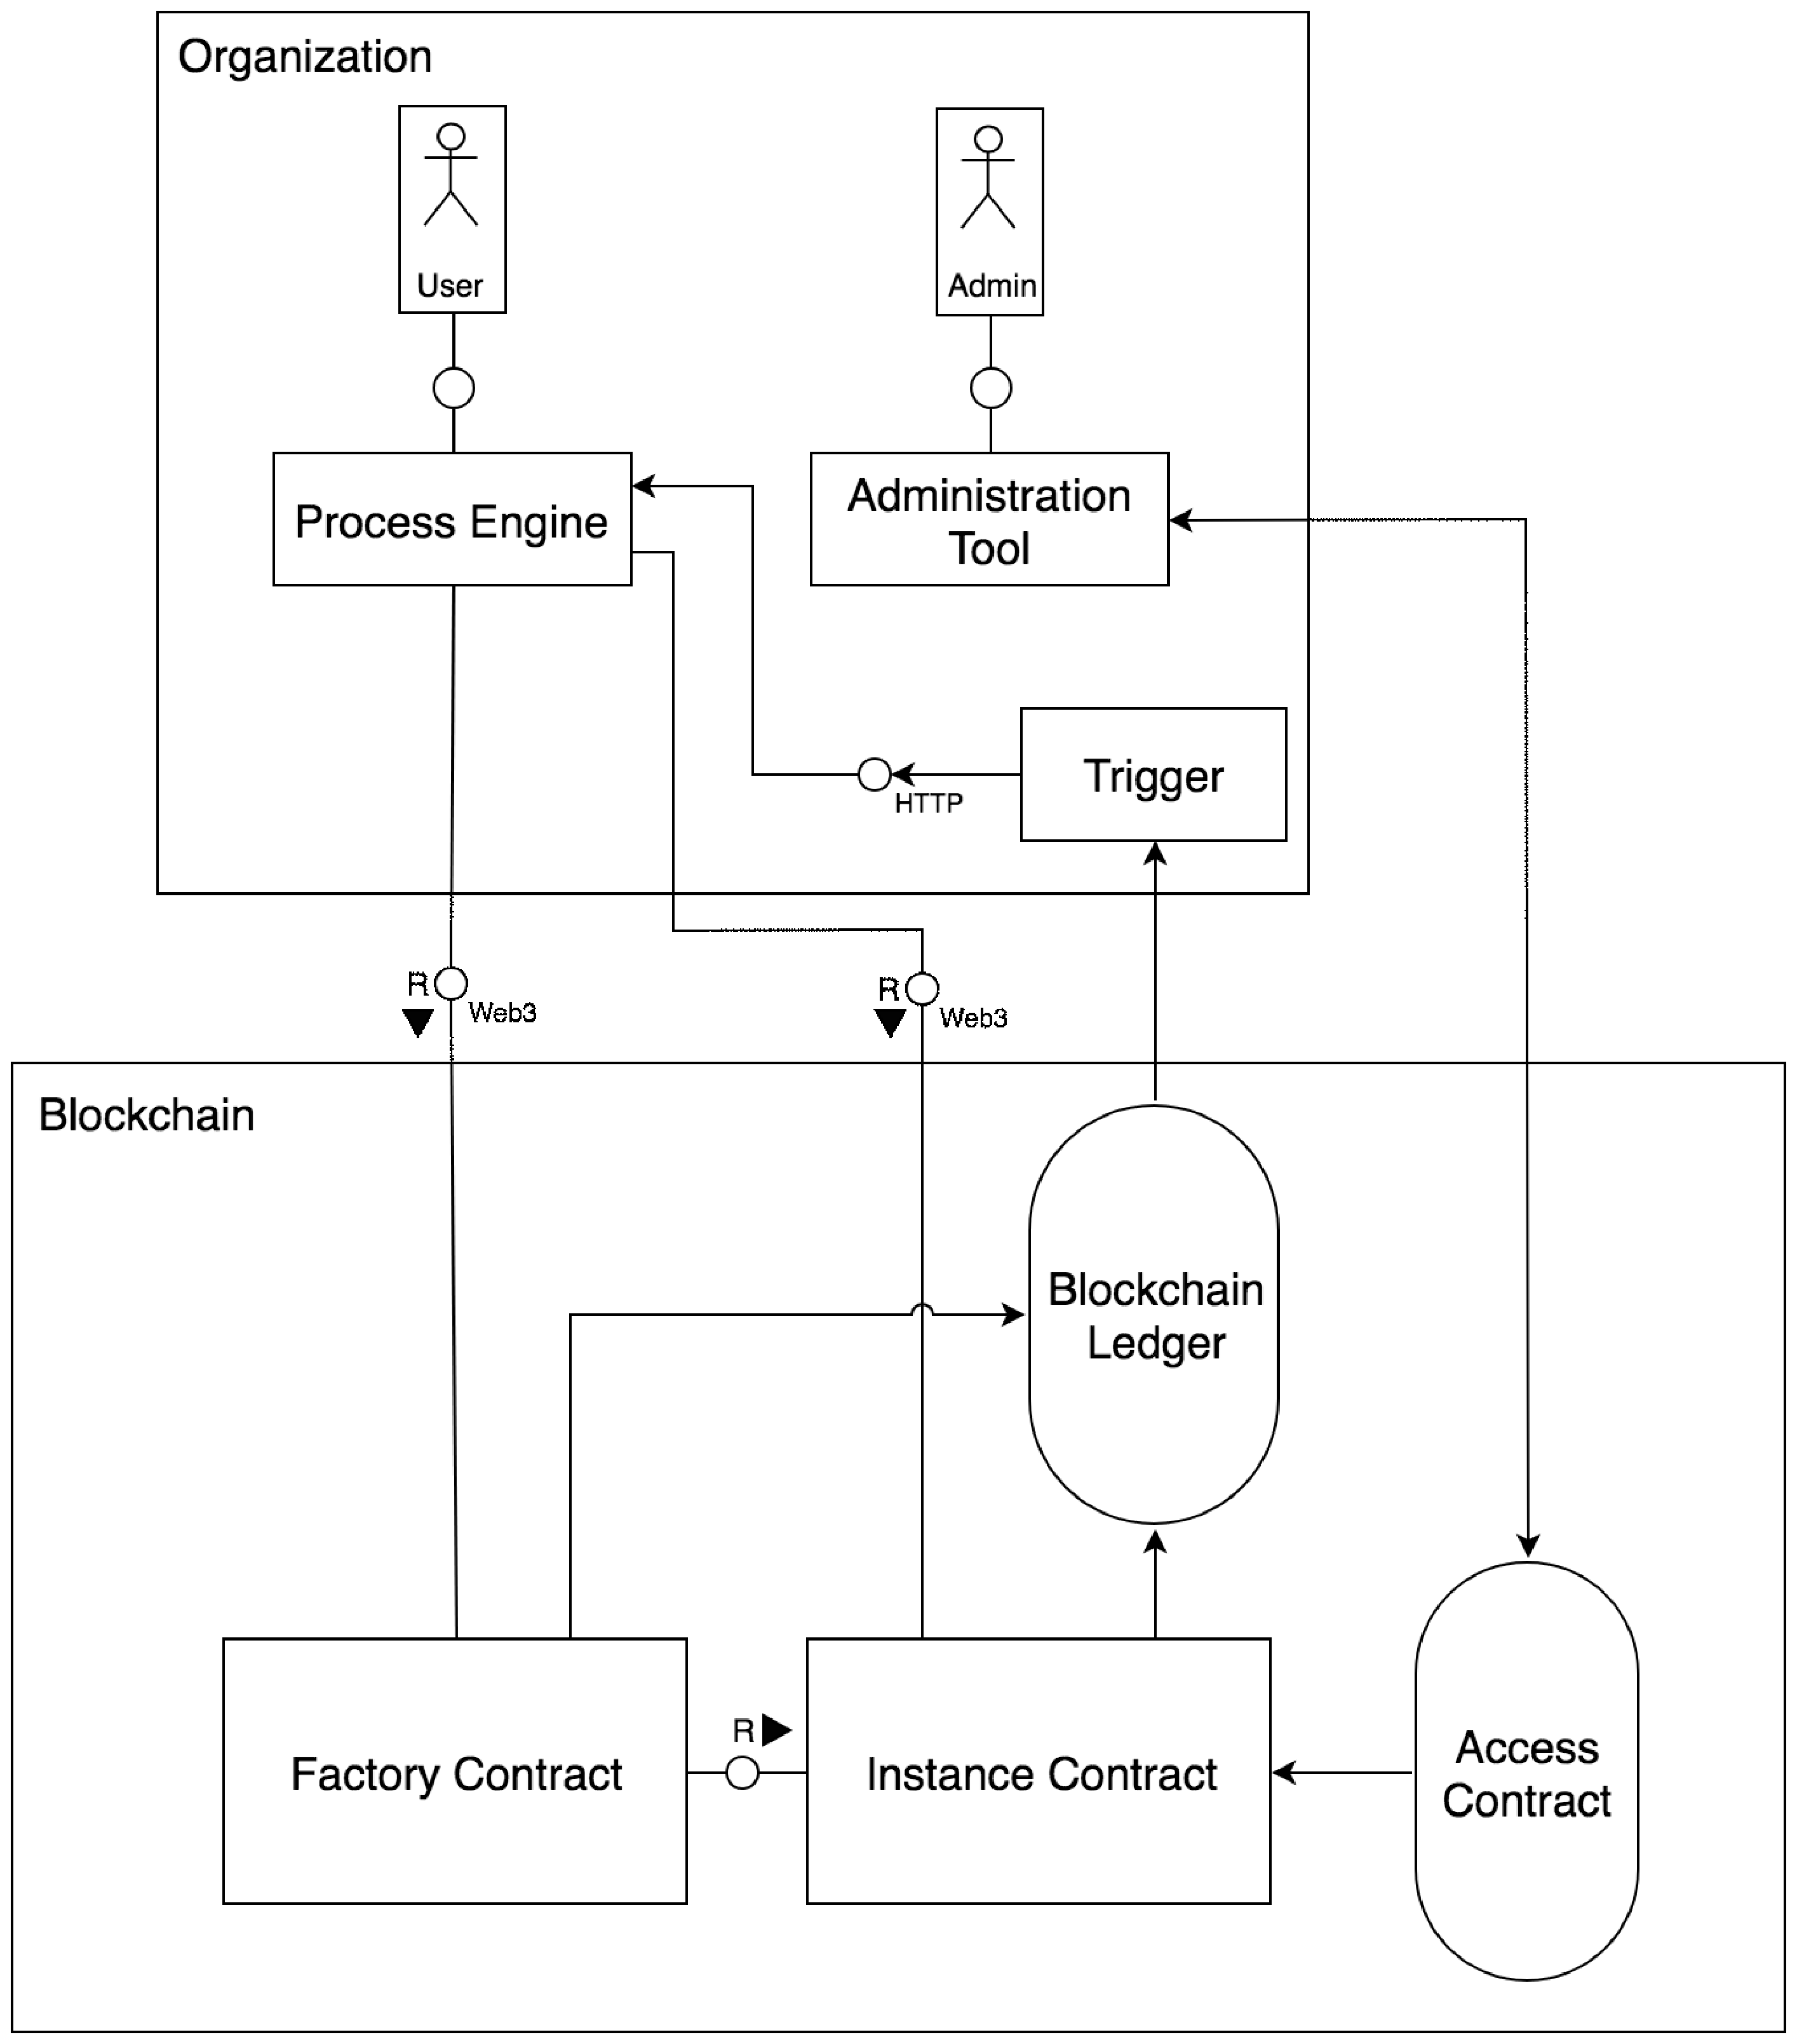
\includegraphics[width=0.6\textwidth]{fig/system_diagram.eps}
	\caption{An architecture diagram showing the interactions within the system.}
	\label{fig:system_diagram}
\end{figure}

Every organization provides an interface of their public process in an \emph{instance contract}.
Additionally, \emph{factory contracts} manage these instance contracts and \emph{access contracts} are used for rights management.
The contract structure will be described in detail in the following sections.
We assume that all participating organizations use a process engine to execute their private processes.
When a throw event is triggered within a process engine, the process engine calls the \emph{throw event function} on an instance contract, which in turn automatically calls the corresponding \emph{catch event function} on the instance contract of the organization responsible for catching the event.
Thus, all communication between organizations is recorded on the blockchain.

Each organization deploys a \emph{trigger} application that continuously listens to catch events (as described in~\cite{weber2016untrusted}).
If a catch event is observed, this information is relayed to the process engine to handle the event.
The usage of the blockchain to monitor the choreography is encapsulated in the process engine and is therefore hidden from the users.

The structure of components for one organization can be seen in Figure \ref{fig:system_diagram}.

\subsection{Contract Structure}
To realize the system, we use three kinds of smart contracts.
Firstly, each organization uses one \emph{instance contract} per process instance.
It represents the public process of the organization for the corresponding process.
It is called during the process execution when a catch or throw event is reached in the process instance.
When this happens, it emits an event on the blockchain to document this fact.

Secondly, each organization uses one \emph{factory contract} per process.
It is responsible for creating instance contracts and saving a mapping from instance IDs to the corresponding contracts.

Thirdly, each organization uses \emph{access contracts} to manage which users can trigger events on the instance contracts.
Either there is one access contract per process or access contracts are shared over multiple processes depending on the use case.

\subsection{Per-Company Setup}
\begin{figure}
	\centering
	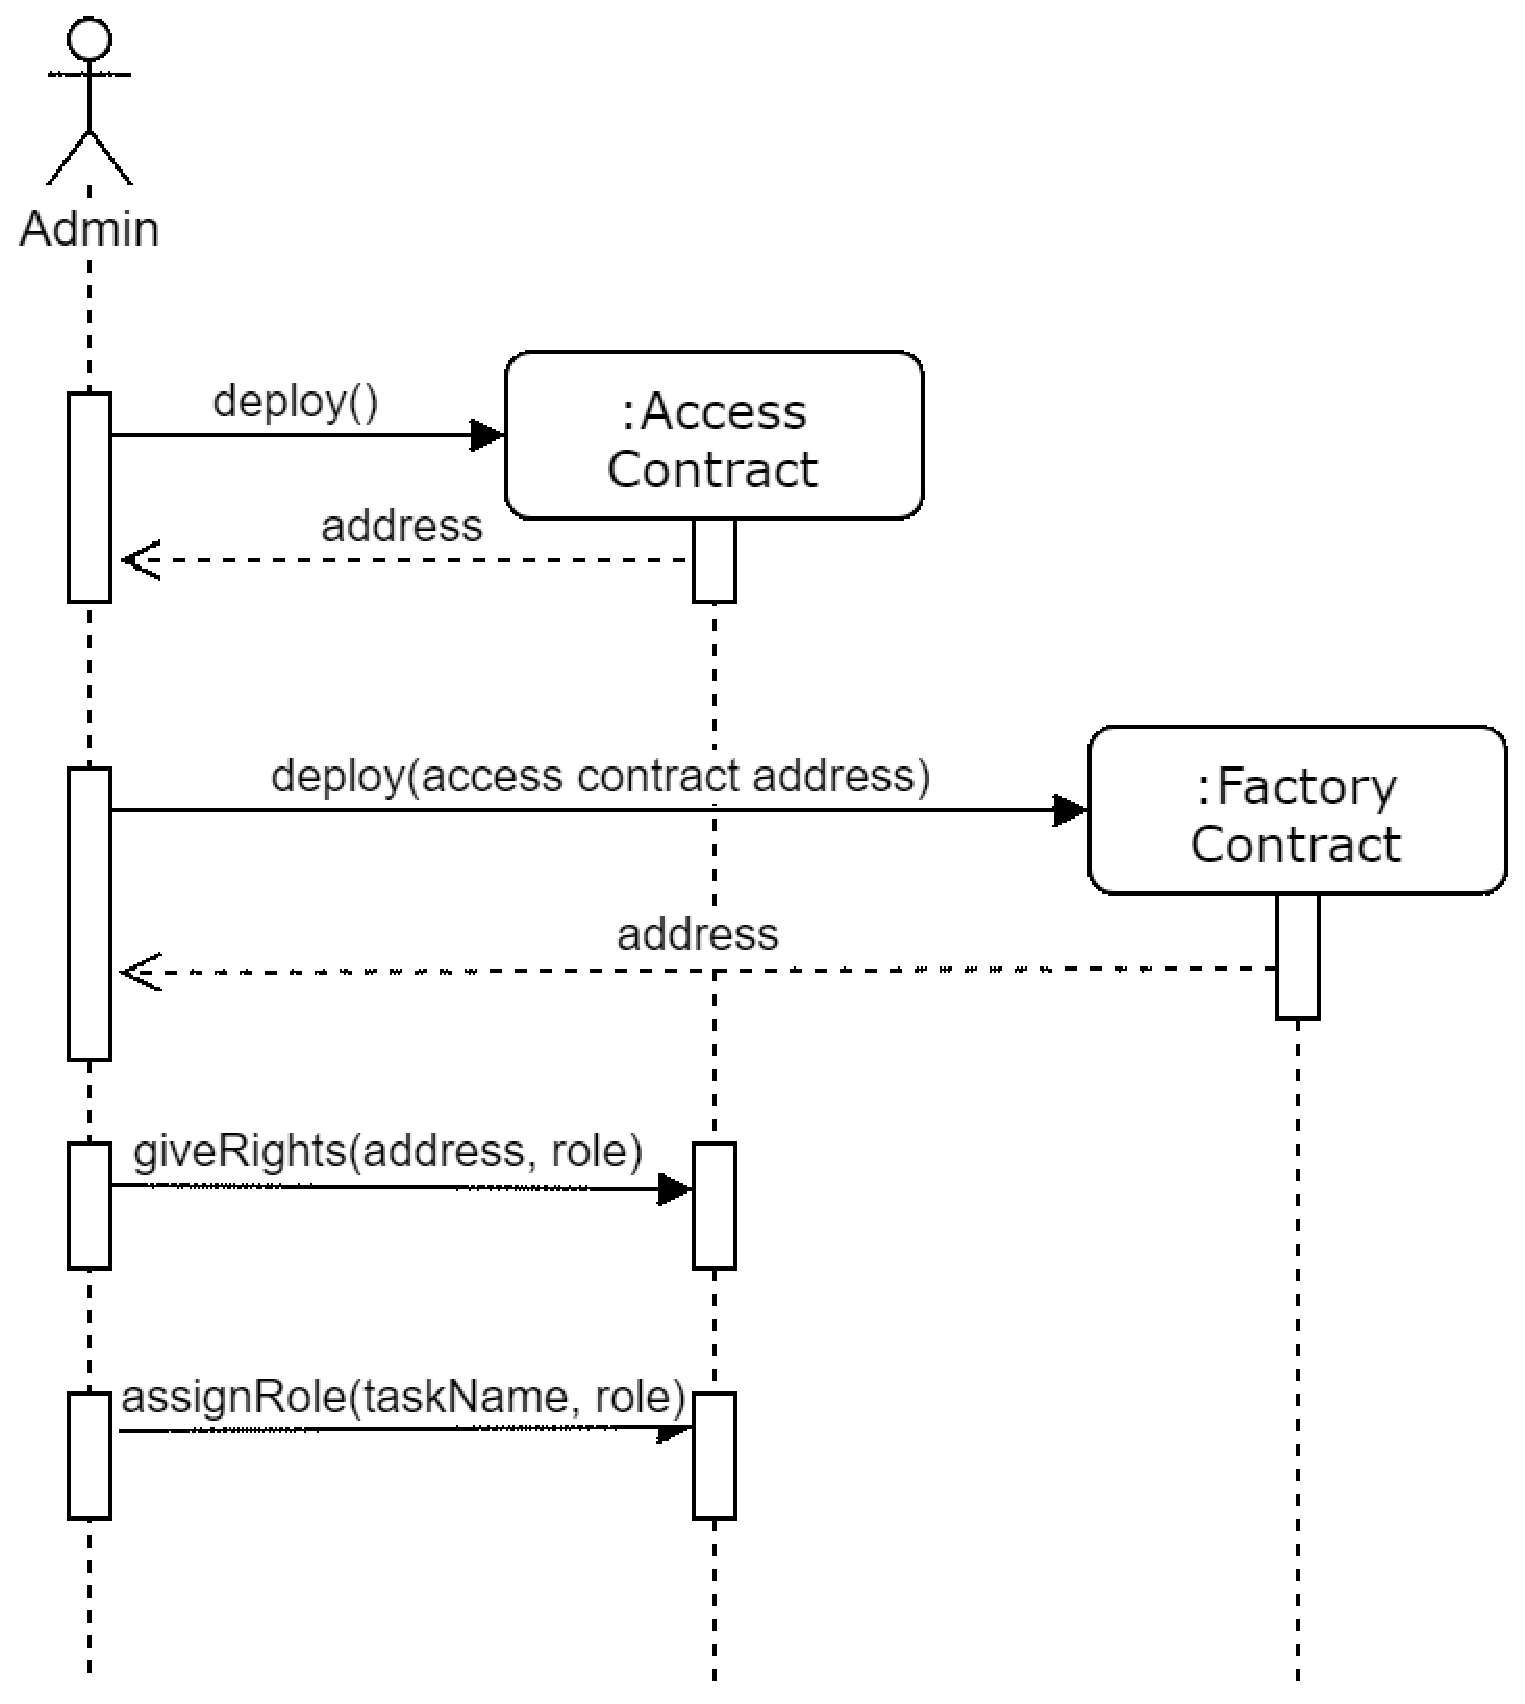
\includegraphics[width=0.45\textwidth]{fig/initialization.eps}
	\caption{A sequence diagram describing the initialization process for an organization.}
	\label{fig:initialization}
\end{figure}

%TODO add a step where other factory contracts are set
Each organization needs to perform some setup before they can take part in a process execution.
An access contract and a factory contract for a process need to be deployed, if it has not been done yet.
Additionally, the user-to-role and and task-to-role mappings have to be updated (via the \emph{giveRights} and \emph{assignRole} functions, respectively), to allow verification of users during the process execution.
A diagram of this process can be seen in Figure \ref{fig:initialization}.

\subsection{Interaction Setup}
\begin{figure}
	\centering
	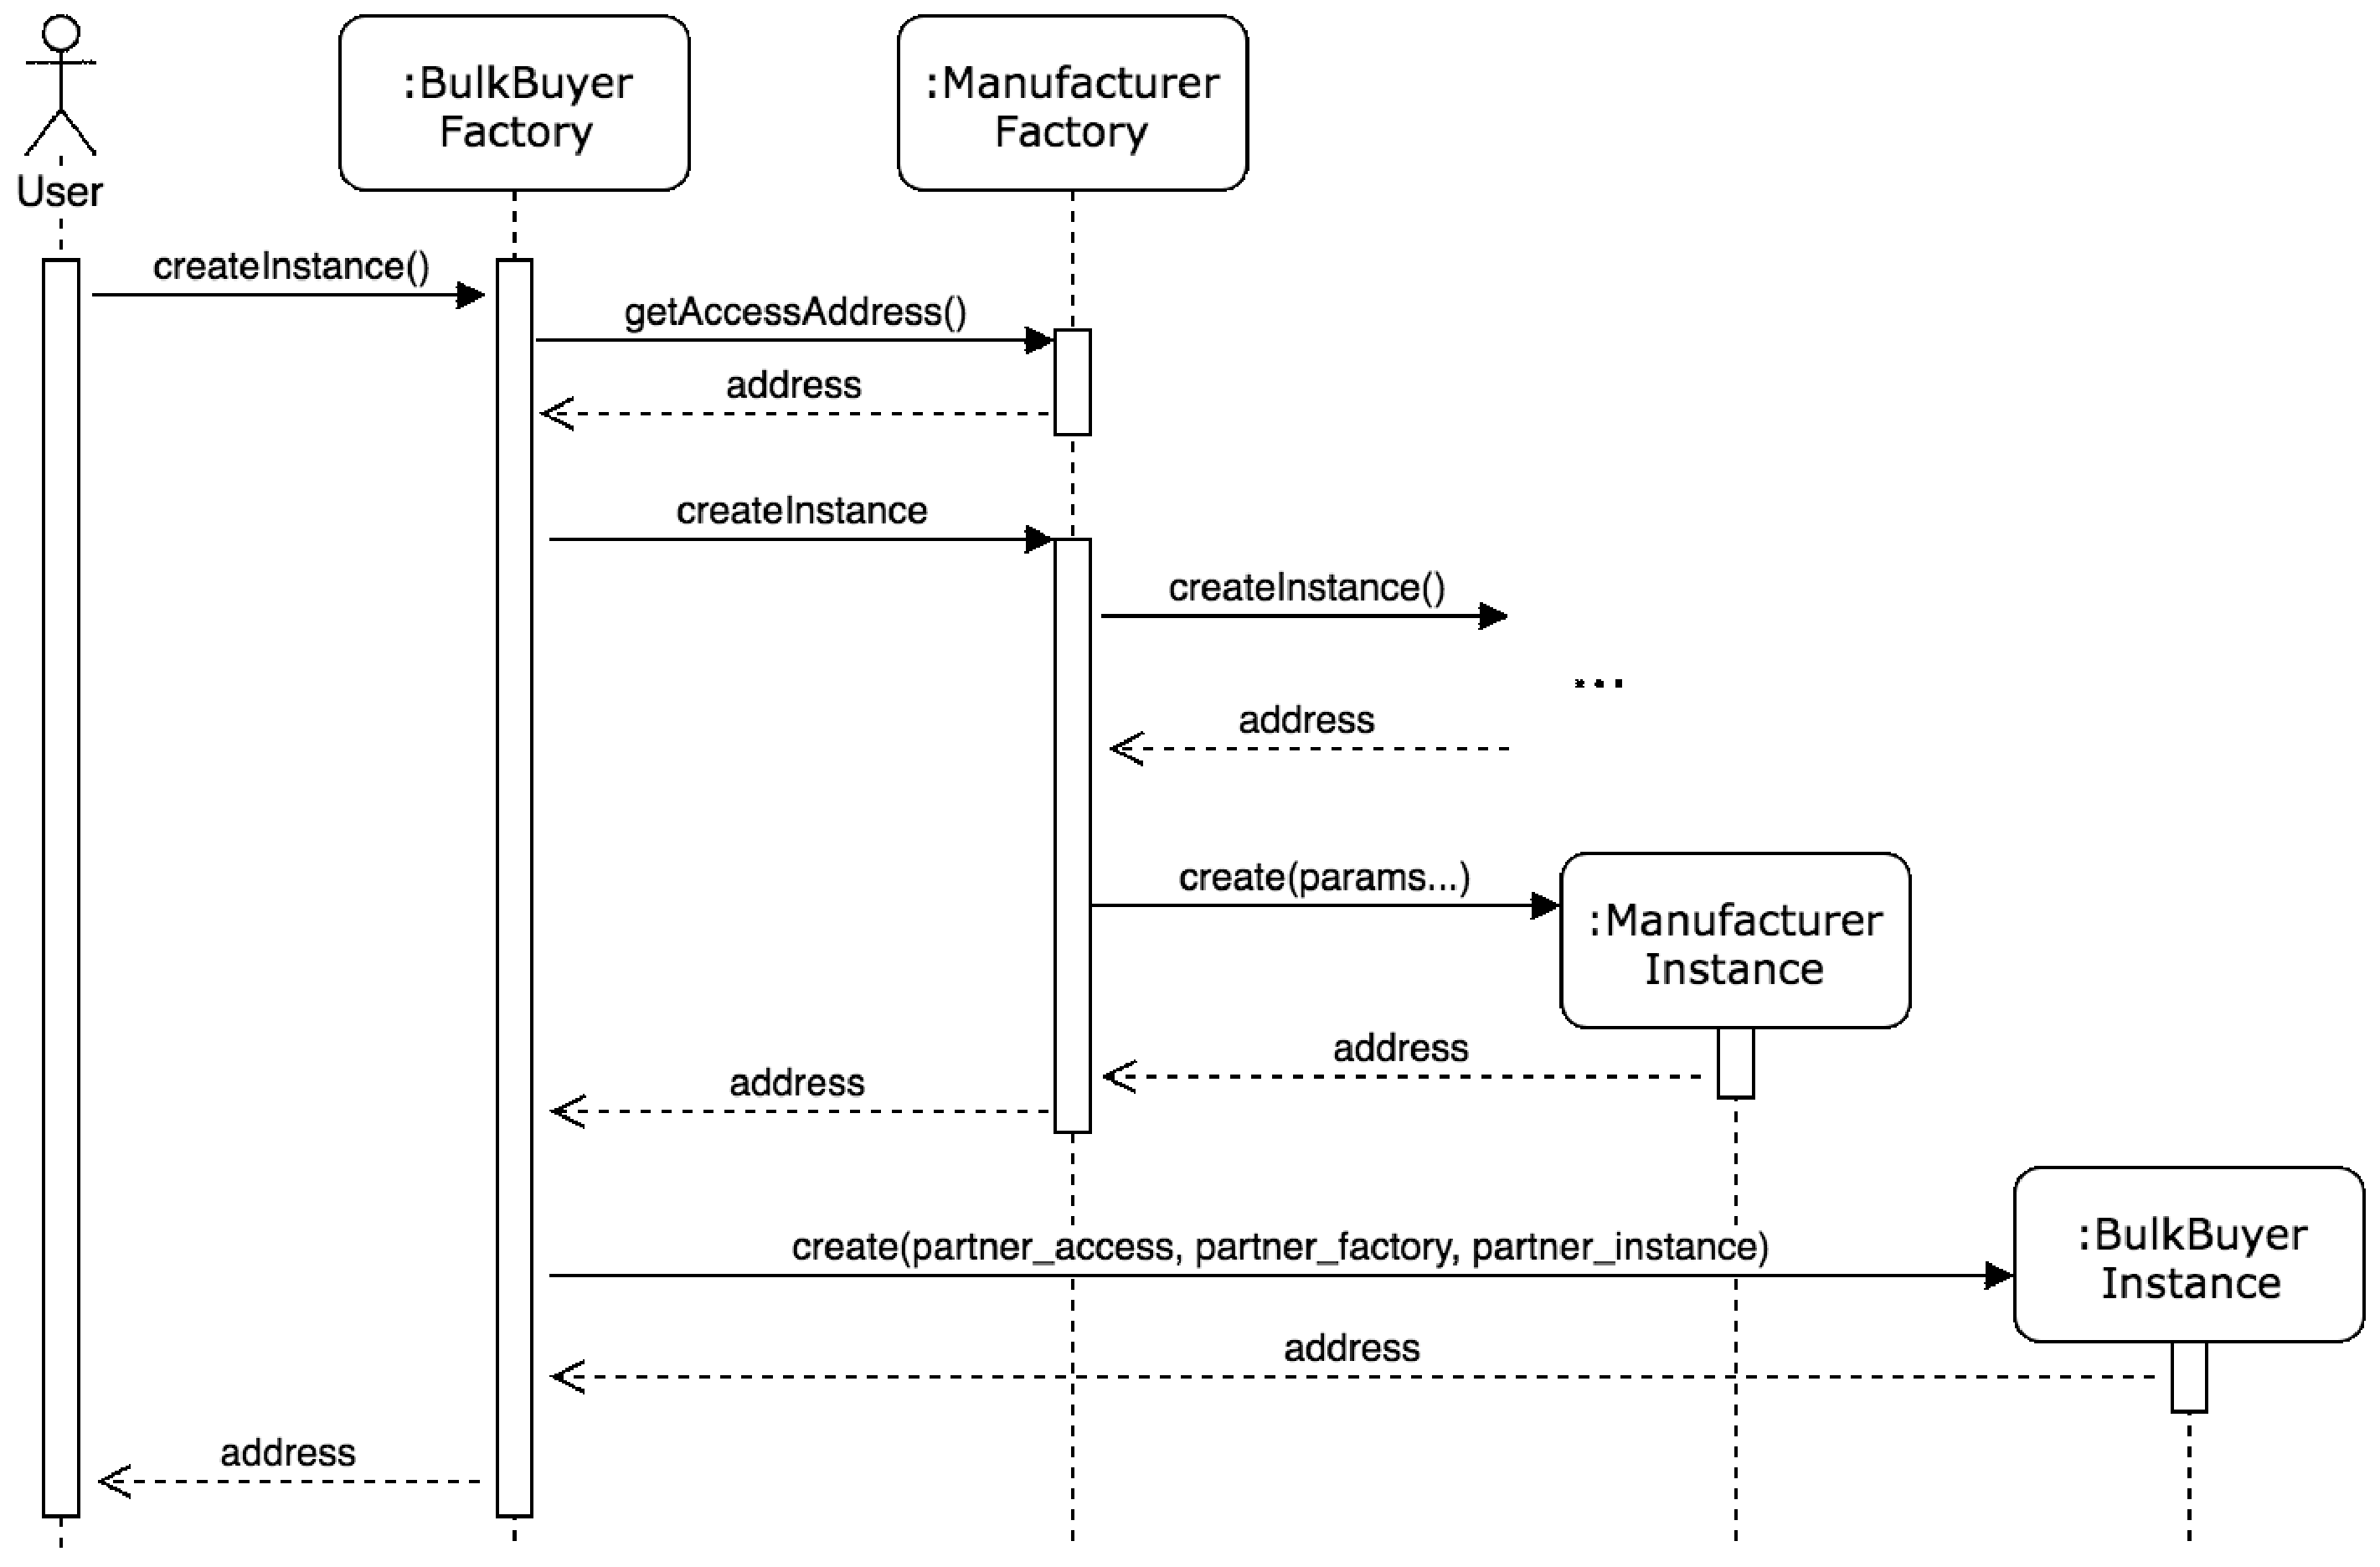
\includegraphics[width=\textwidth]{fig/instance_creation.eps}
	\caption{A sequence diagram describing the process of creating a new process instance.}
	\label{fig:instance_creation}
\end{figure}

In order to create a new process instance, the organization that initiates the instance by triggering the first throw event has to explicitly create an instance contract by calling the factory contract.
To create an instance contract, the factory contract may need to initialize other instance contracts by calling other factory contracts.
When all partner instance, factory and access contracts are known, the instance contract can be created and its address is returned to the user and an event is emitted to the blockchain.
This process is visualized in Figure \ref{fig:instance_creation}.

The recursive initialization ensures that all instance contracts that are part of the process instance will be created by one function call.
%TODO add emit event in the diagram
%TODO better formulation
The organizations that did not start the instance creation can detect the new process instance by using their trigger to watch the factory contract.

\subsection{Sending Messages}
\begin{figure}
	\centering
	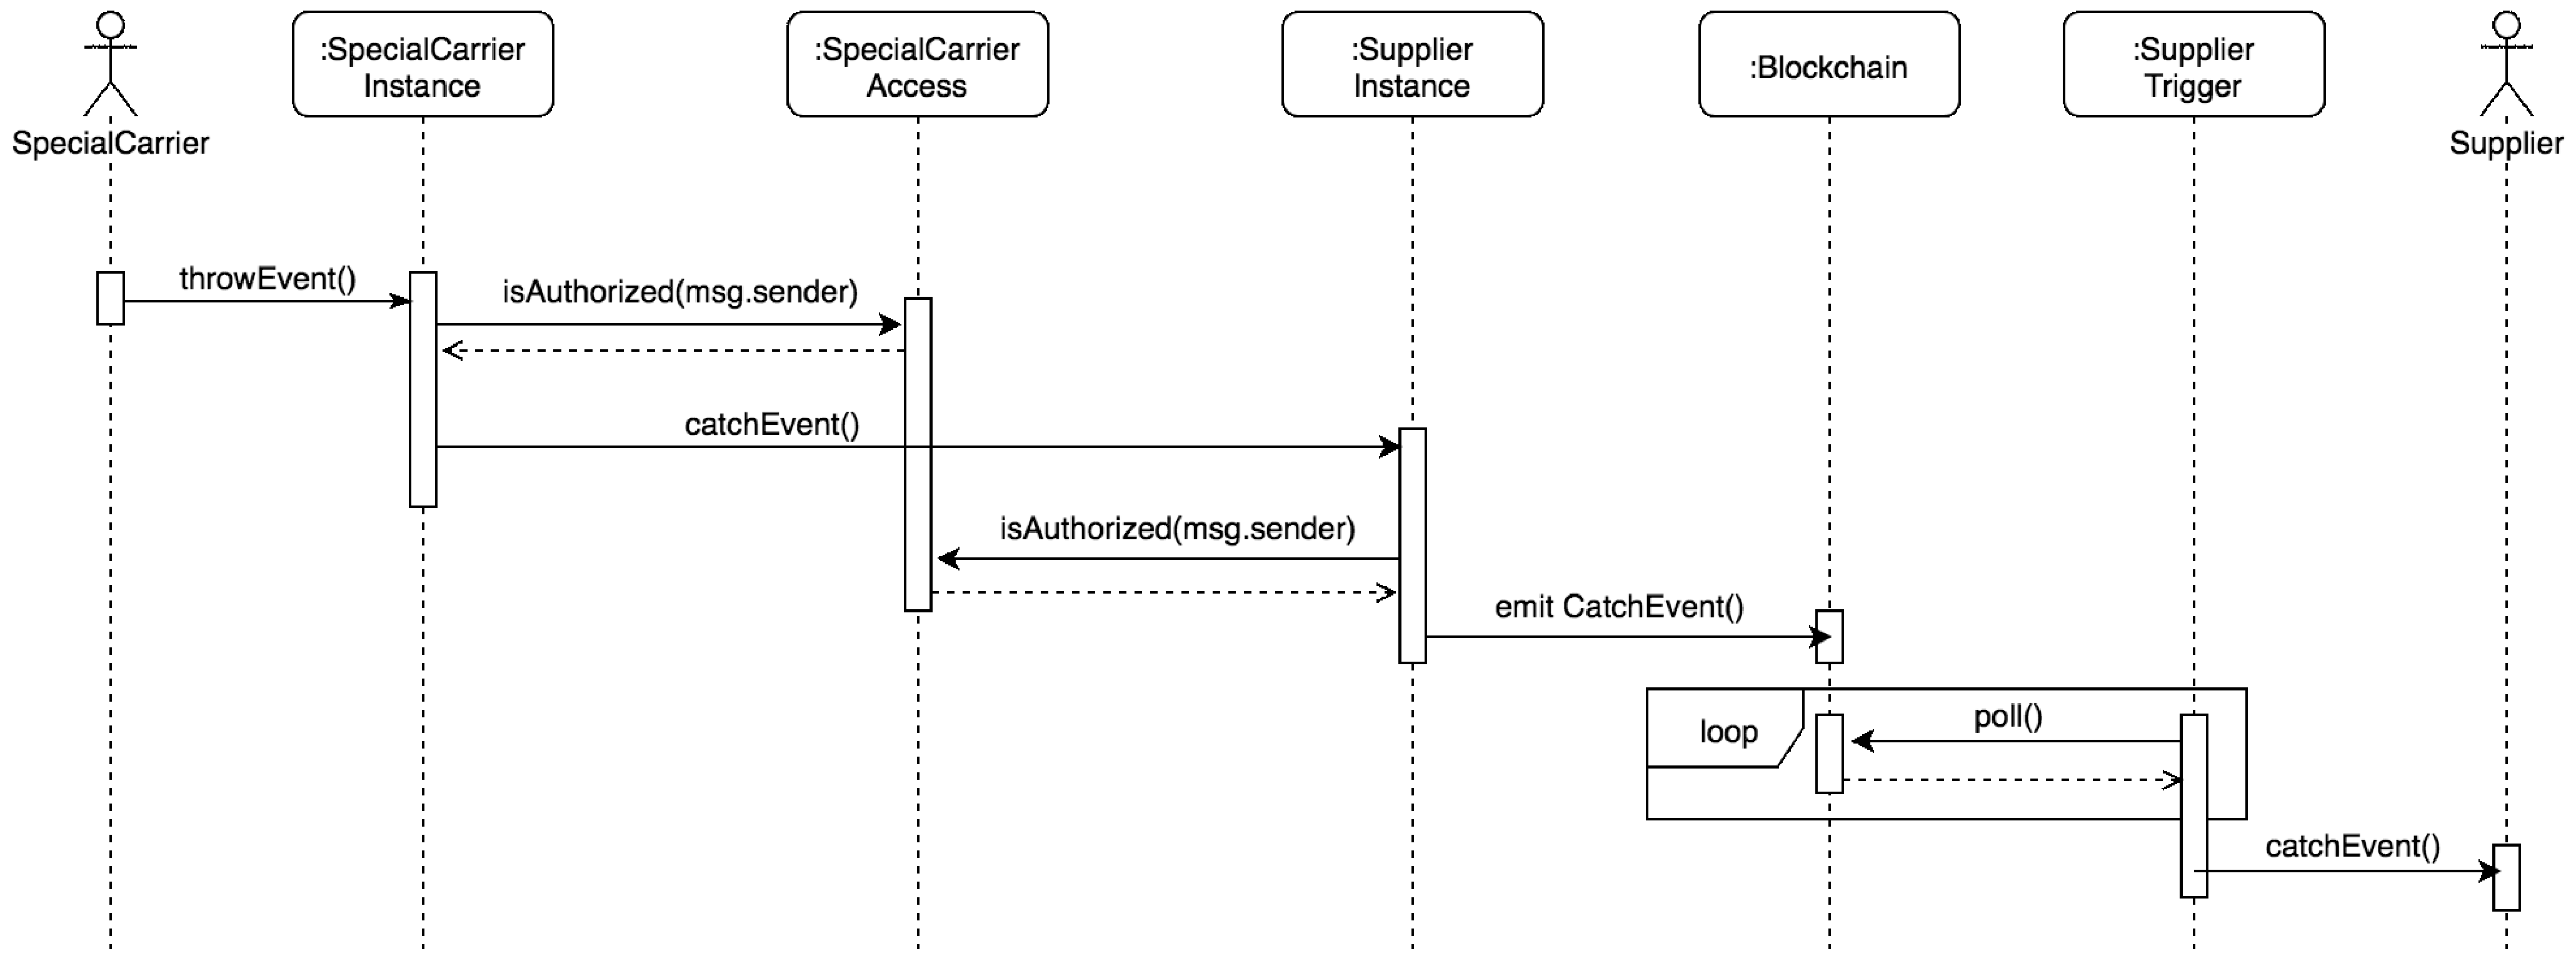
\includegraphics[width=\textwidth]{fig/event_sending.eps}
	\caption{A sequence diagram describing the process of sending a message to a collaboration partner.}
	\label{fig:event_sending}
\end{figure}

%TODO correctly show that the address is passed instead of using msg.sender
When a throw event is triggered in the process engine of organization $A$, the process engine of $A$ calls the corresponding \emph{throw event function} on the instance contract of organization $A$.
In the instance contract of $A$ an authorization is performed by looking up the sender address in the access contract of $A$.
If this check is successful, the \emph{catch event function} is called on the partner instance contract of $B$.
In the instance contract of $B$ there is another authorization against the access contract of $A$.
This ensures that both sides can be confident, that the throw event was triggered by an authorized person who belongs to organization $A$.
If this check was also successful, an event is emitted to the blockchain.
This will be detected by the trigger of $B$ and passed to the process engine.
Thus, a message was sent from $A$ to $B$ via the blockchain and an audit trail was created.
An example can be seen in the sequence diagram in Figure \ref{fig:event_sending}.
% TODO explain how payload could look like

\section{Implementation} \label{implementation}

Given the architecture, we will now discuss the implementation of the contracts used in the system.
Afterwards, we will shortly describe the tools we built for interacting with the system.

\subsection{Contracts}

In the following, we will formally describe our contract implementations.
The implemented contracts can be found in our repository at \url{https://github.com/p-otto/ProcessesMeetBlockchain2018/tree/master/armadillo/resources}.
% TODO repo ist noch private
% TODO update if repository changes

\subsubsection{Process Contracts}

For taking part in the process collaboration, each company needs to deploy a factory contract that is responsible for creating instance contracts.
To this end, the factory contract source code needs to contain the definition of the company's instance contract.
This closely follows the factory contract pattern used in~\cite{weber2016untrusted}, and described as pattern 14 in~\cite{xu2018pattern}.

In our implementation, a company's factory contract also knows the address of the company's access contract for convenience.
Additionally, it stores the addresses of created instances, mapped by a \emph{choreography instance ID}, i.e., an ID that is shared between all choreography participants for each instance of the shared choreography.

To allow interaction between companies via the blockchain, two participants need to exchange the addresses of their factory contracts when there is a direct interaction between them.

A factory contract thus has the resulting interface:
\begin{itemize}
	\item A \texttt{constructor} where the address of the company's access contract is passed
	\item Setter methods for the factory contract addresses of interaction partners
	\item A \texttt{createInstance} function
	\item A \texttt{getAccessAddress} function
	\item A \texttt{isInstance} function used to verify whether an address points to an instance contract created by this factory (for a given choreography ID)
\end{itemize}

Internally, there are a few implementation details worth mentioning.
Regarding storage, private fields are necessary holding the factory contract addresses, the access contract address as well as the instance address mapping.
To avoid communication errors at runtime, it should not be possible to call \texttt{createInstance} before all required factory addresses are set.
Finally, there is one minor implementation difference depending on whether a participant is the \emph{choreography initiator} (the participant to manually start the choreography instance by sending a request):
The initiator needs to generate the choreography instance ID inside of its \texttt{createInstance} function, and pass it to all its interaction partners.
Every other participant needs to have a parameter for the ID in their \texttt{createInstance} function.

Communication between smart contracts happens in the form of function calls.
To allow the factory and instance contracts to call functions on their interaction partner's contracts, the partner's function interface needs to be known, i.e., it needs to be declared in the factory contract source code.
%- the access contract (same for every participant)
%- remote factory contracts (if receiving messages from remote, for verification)
%- remote instance contracts (if sending messages to remote instance)

The instance contract definition is also part of the factory contract source code.
The factory contract creates an instance by calling its constructor and passing all for the inter-process communication required addresses.
Instance contracts provide functions for each sending action, i.e., send tasks or events in the company's process, which can be called by the process engine.
For each receiving action (task or event), a function needs to be present that can be called from other instance contracts.
When company $A$ triggers a sending function on their instance contract, it in turn calls a corresponding receive function on the instance contract of company $B$.

Instance contracts need to store:
\begin{itemize}
	\item The choreography instance ID for verifying incoming messages
	\item The addresses of the factory and access contracts of partners for verifying incoming messages
	\item The addresses of the instance contracts of partners for sending messages
	\item The address of the company's own access contract, for verifying local function calls
	\item The address of the company's own factory contract, for returning any remaining funds upon \texttt{selfdestruct}
\end{itemize}

A few more implementation details are worth noting:
Verification is implemented on sender-side and on receiver side.
Each send function has a guard checking the caller in the company's own access contract.
Each receive function has a guard checking a) that the caller is a contract instance that is part of the choreography instance (via the partner factory contract), and b) checking the account behind the request in the partner's access contract.
Guarding functions against unwanted access was described in pattern 13, Embedded Permission, in~\cite{xu2018pattern}.

Having achieved a traceable communication on the blockchain using contract function calls, we still want to access messages in off-chain applications, e.g., triggering process events in a process engine on message receive.
To this end, smart contracts need to implement events that are emitted to the blockchain whenever a receive function is executed.
Blockchain events can then be watched, and reacted upon, by off-chain components.

In our current implementation, the end of a process instance is marked by the instance contract selfdestructing.
At the end of the execution of the last send or receive function in the process, the solidity builtin \texttt{selfdestruct} is called.
By passing the factory contract address, potential remaining funds are transferred to the factory contract.

\subsubsection{Access Contract}

Each company deploys an access contract that holds information about the roles and permissions of the company's employees.
Having permission data encapsuled in a separate access contract follows pattern 12, the Data Contract pattern, from~\cite{xu2018pattern}.
It allows decoupling the roles and permissions from the actual contract instances, allowing for a simple modification at runtime.
Access contracts can be deployed per process, or even once per company as a single source of truth for all processes.

To allow the administration of user permissions, access contracts provide the following interface:
\begin{itemize}
	\item \texttt{assignRoleToUser(userAddress, role)}
	\item \texttt{removeRoleFromUser(userAddress, role)}
	\item \texttt{assignTaskToRole(task, role)}
	\item \texttt{removeTaskFromRole(task, role)}
\end{itemize}
The access to these functions should be guarded, allowing only a specific administrator address to call them.

Verifying a users permission to execute a certain task can be achieved by calling \texttt{isAuthorized(userAddress, task)}.
\newline

Given this interface, there are multiple possible implementation approaches for access contracts.
As it was our main focus to develop a running prototype, and not to provide an optimized, production-ready system, we decided on a simple mapping-based implementation:
\begin{lstlisting}[
  caption=Mappings in our access contract implementation,
  language=Solidity
]
pragma solidity ^0.4.23;

contract Access {
    mapping(string => string) taskToRole;
    mapping(string => uint) roleToIndex;
    mapping(address => uint) addressToAccessBitmask;
    ...
}
\end{lstlisting}
The first mapping stores the tasks that can be executed by a specific role (cf. pools and lanes, and their contained tasks, in BPMN diagrams).
The second mapping assigns each role an index in the access bitmask, i.e., if the bit at the given index is set, the user holds the corresponding role.
The third mapping assigns such an access bitmask to each user.

Storing large amounts data on the blockchain is expensive by design.
As the mappings grow in size with each user, role and task that is part of some process in the company, our implementation is probably not suited for real-world application.
Finding optimized, less costly (both in computation cost and storage cost) approaches is part of future work.
One other approach we thought of is based on pattern 5 of~\cite{xu2018pattern} - depicting real world permissions as tokens, and "paying" with these tokens on function call to verify one's role.

\subsection{Tools}

In the following, we will briefly present the tools we implemented integrate process management with our blockchain approach.
The implementations can be found in our repository at \url{https://github.com/p-otto/ProcessesMeetBlockchain2018/}, in the \texttt{armadillo} and \texttt{eth\_admin} folders, respectively.
% TODO repo ist noch private
% TODO update if repository changes
% TODO overfull hbox


\subsubsection{Armadillo}

\begin{figure}
	\centering
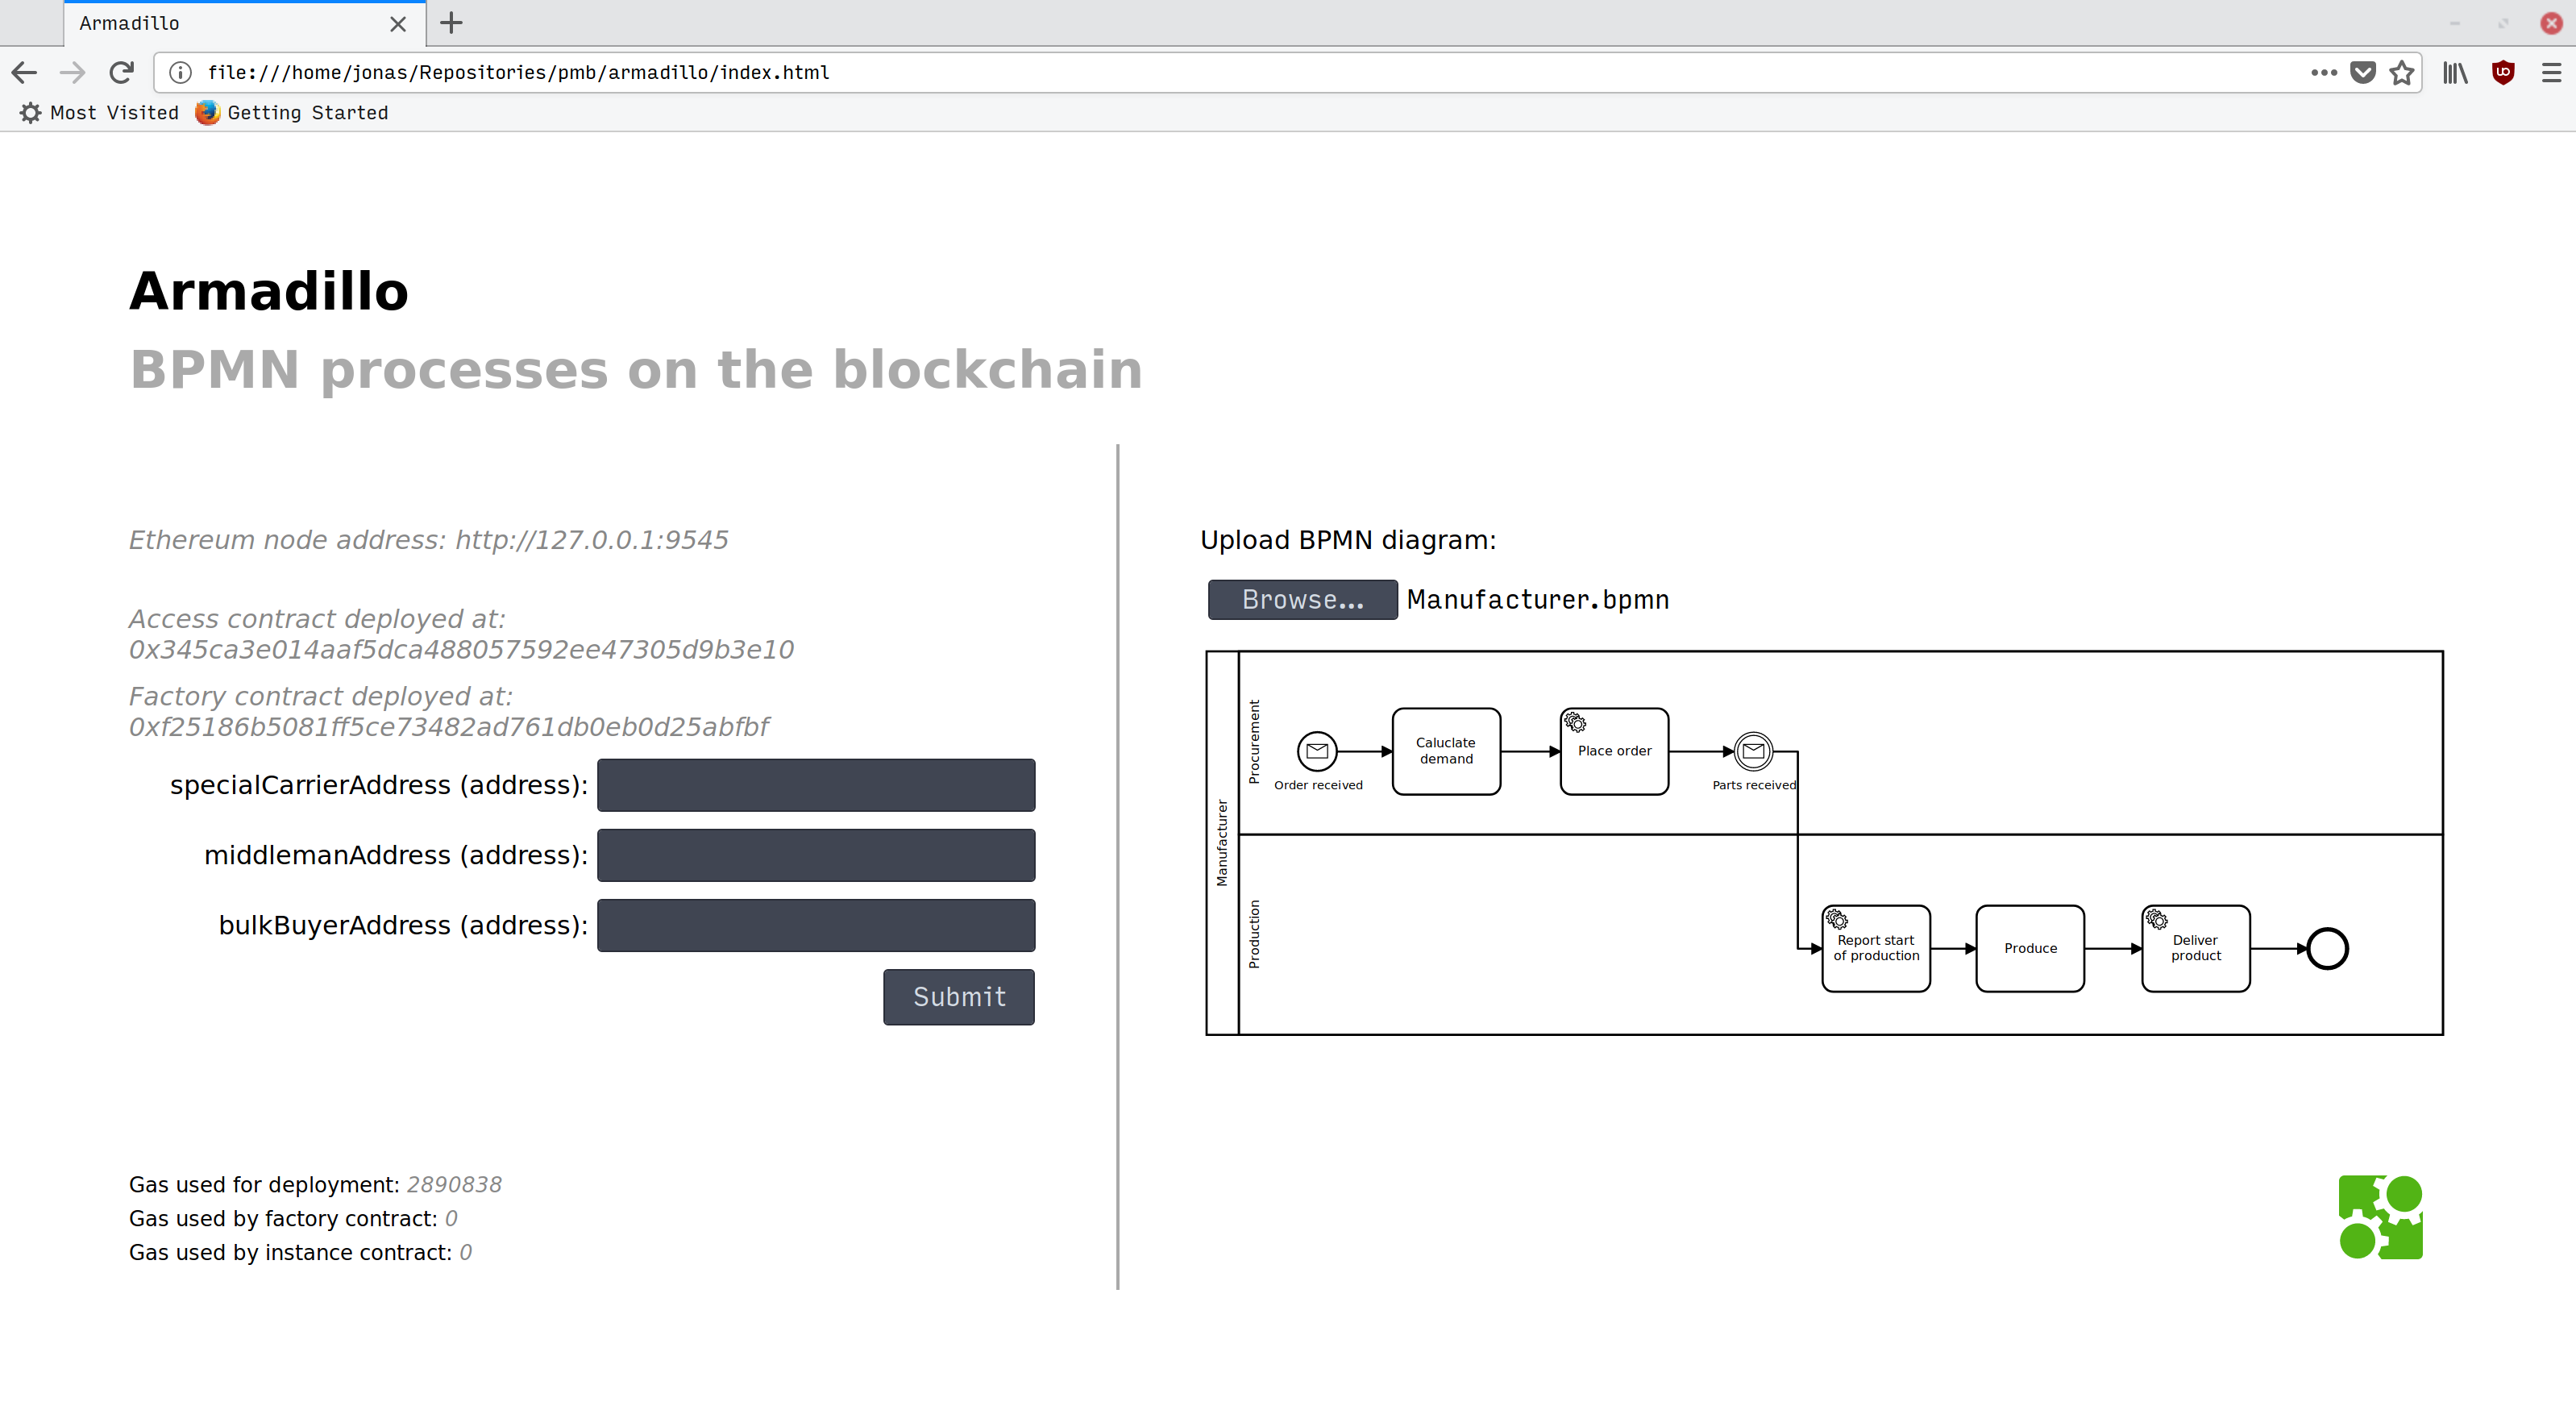
\includegraphics[width=0.9\textwidth]{fig/Armadillo.png}
\caption{Screenshot of the Armadillo web application.}
\label{fig:armadillo}
\end{figure}

As a way of joining process execution with our blockchain architecture, we developed a single page web application (see Figure \ref{fig:armadillo}) in JavaScript and HTML, using the Vue.js framework\footnote{\url{https://vuejs.org}}.
With the help of the Web3 Ethereum JavaScript API\footnote{\label{web3}\url{https://github.com/ethereum/web3.js/}}, we can trigger contract functions based on user actions in the applications user interface.
Armadillo also implements the upload and rendering of BPMN diagrams using the bpmn.js toolkit\footnote{\url{https://bpmn.io/toolkit/bpmn-js/}}.
Building upon the BPMN viewer provided in the toolkit, we implemented the handling of user clicks on \emph{BPMN Service Tasks}, which allowed us to use the viewer as a process engine mock.
A screencast of the full choreography can be found in the respository under \url{https://github.com/p-otto/ProcessesMeetBlockchain2018/blob/master/presentation/armadillo-screencast.mp4}.
% TODO repo, hbox etc.

\subsubsection{Eth\_Admin}

We developed a small command line application for managing users and roles via the access contract.
The application is written in JavaScript in the node.js framework\footnote{\url{https://nodejs.org/}}.
Internally, calls functions on access contracts utilizing the Web3 Ethereum JavaScript API\textsuperscript{\ref{web3}}.
We decided to build the command line functionality with the help of the Vorpal framework\footnote{\url{http://vorpal.js.org/}}.
The \texttt{README} in our repository describes how to use the application.

\section{Discussion} \label{evaluation}

When evaluating blockchain implementations, the underlying system comes with new aspects that need to be considered.
First, computation and data storage on the blockchain needs to be paid for in \emph{transaction fees}.
In Ethereum, the unit \emph{gas} was introduced as a way of having consistent fee pricing in spite of fluctuating Ether prices.

We measured the gas used for each transaction that is executed by the Armadillo tool, and we summed up the gas usage for the different kinds of contracts in the companies in Table \ref{gasusage}:

\begin{table}
	\centering
	\caption{Gas used by contracts in the example choreography.} \label{gasusage}
	\begin{tabular}{|l | c | c | c|}
		\hline                          & \textbf{Factory} & \textbf{Instance} & \textbf{Sum}       \\
		\hline \textbf{Bulk Buyer}      & 4,590,569        & 59,396            & 4,649,965          \\
		\hline \textbf{Manufacturer}    & 129,588          & 124,316           & 253,904            \\
		\hline \textbf{Middleman}       & 129,586          & 111,189           & 240,775            \\
		\hline \textbf{Supplier}        & 86,398           & 61,745            & 148,143            \\
		\hline \textbf{Special Carrier} & 86,376           & 81,945            & 168,321            \\
		\hline \textbf{Sum}             & 5,022,517        & 438,591           & \textbf{5,461,108} \\ \hline
	\end{tabular}
\end{table}
% TODO add exchange rates and $ price? or propmt users to look it up themselves because of changing gas price?
Most of the transactions have proven to come with reasonable gas costs.
However, the instantiation cost that is currently paid by the initiator appears to be problematic.
As the first instantiation transitively triggers all the other participant's instantiations, this can become quite costly, and might even surpass the \emph{block gas limit}, the maximum amount of gas that can be spent per new block, depending on the number of participants involved.
%Even if that is not the case, a high gas cost is still a problem, since in Ethereum, by design, transactions with high gas costs are less likely to be included in a block by miners, possibly leading to long waiting times. % TODO why again?

Second, security is one of the main reasons to opt for blockchain systems.
In our case, we put effort into making the message exchange secure by adding multiple steps of access verification using the access contracts.
Access contracts themselves, however, only implement access verification by comparing the sender address with the address the contract was deployed with (the \emph{owner} address).
As the owner can give and remove access rights freely, another layer of off-chain security might make sense here to restrict the owner account from unwanted access.

\section{Future Work} \label{futurework}

We researched a system prototype for handling process choreographies on the blockchain.
While we were able to execute an example choreography using our implementation, a few aspects are left for future work.

\subsubsection{Instantiation Costs}

During evaluation, we saw that the instantiation costs are very high, have a potential to hit the gas limit in larger choreographies and also have to be paid by the initiator.
These problems need to be addressed before our solution is feasible for production use.
Further research thus could be invested into a more decentralized instantiation, where each participant pays for its own instance contract creation.
One apporach worth considering is to have the intiator emit a specific instance creation event that each other participant would listen to.
The process engine could then react to such an event with the help of a trigger, and call the \texttt{createInstance} method.
Then the other factory would have to be notified that the instantiation was successful.

\subsubsection{Access Contract}

As stated earlier, there probably are better ways of implementing role-based access control in a smart contract.
We decided for a simple mapping-based approach, which requires large amounts of memory.
Finding approaches that are more suited for blockchain architectures is one direction in which further research could go.

\subsubsection{Process Contract Generation}

Our contract implementations are the result of manual, iterative development.
Having reached the final iteration, we realized that the contracts share common patterns.
Most of the implementation could probably be generated, i.e., from a choreography diagram (or at least from the participant's public processes).
The next step would be to define a template for the factory contract source code, to determine which parts are easily generated, and which parts might need manual adjustments, e.g., depending on whether the participant is the initiator or not.
Given such a template, one could work on a contract generation tool that takes a diagram as input and produces factory contract code.
A possible implementation could use a rule-based approach for translating the choreography model, similar to~\cite{lopez2017caterpillar}.

\subsubsection{Process Engine Integration}

In related work~\cite{lopez2017caterpillar}, process logic was executed on the blockchain.
As we decided for a hybrid approach, using a process engine for execution and the Ethereum blockchain for traceable message passing, we implemented a mock process engine in our application.
Now, it certainly makes sense to integrate the system with a productive process engine implementation, e.g., the Camunda BPMN Workflow Engine\footnote{\url{https://camunda.com/products/bpmn-engine}} for further evaluation.

\section{Conclusion} \label{conclusion}

In this paper, we presented a system architecture and prototypical implementation for connecting process execution with blockchain technology.
While keeping the process execution off-chain, we developed an approach of inter-process communication using the Ethereum blockchain as a messaging channel.
Having a permanent ledger as the underlying data structure storing messages, faults and misunderstandings can be traced back to their origin and responsibilities are disclosed.

Building on the findings of this paper, improvements regarding runtime and execution costs open up a wide area of possible future work on the topic.

Currently, blockchain technology is most widely used to handle monetary transactions.
Instead of shifting assets between partners, however, we are using the blockchain to shift \emph{responsibilities}.
Given the similar nature of the two, we speculate that this topic is of future relevance.
%
% ---- Bibliography ----
%
% BibTeX users should specify bibliography style 'splncs04'.
% References will then be sorted and formatted in the correct style.
%
\bibliographystyle{splncs04}
\bibliography{references}

\end{document}
